\section{The Fourier and Wavelet Transforms}

  Computer vision is an extremely difficult task. Greyscale intensities in an image are
  not very helpful in understanding what is in that image. Indeed, these values are
  sensitive to lighting conditions and camera configurations. It would be easy to
  take two photos of the same scene and get two vectors $x_1$ and $x_2$ that have
  a very large Euclidean distance, but to a human, would represent the same
  objects. What is most important in an image are the local variations
  of image intensity. In particular, the location or phase of the waves that make
  up the image. A simple experiments to demonstrate this is shown in 
  \autoref{fig:lena_morph}. 

  \begin{figure}
    \centering
      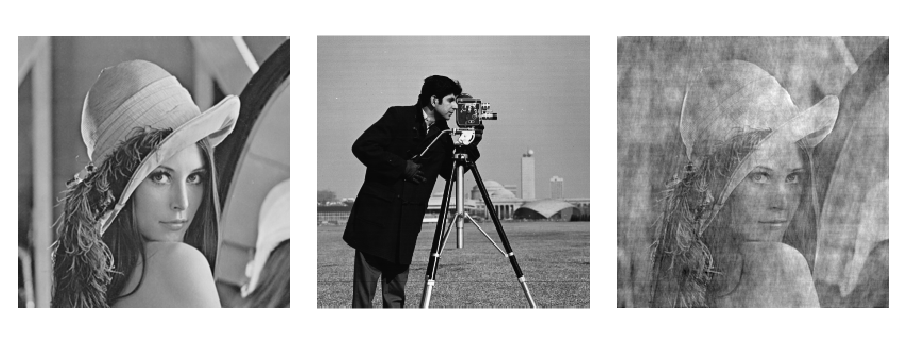
\includegraphics[width=1.1\textwidth]{litreview/images/lena_mag_swap.png}
      \mycaption{Importance of phase over magnitude for images}
        {The phase of the Fourier transform of the first image is combined 
         with the magnitude of the Fourier
         transform of the second image and reconstructed. Note that the
         first image has entirely won out and nothing is left visible of
         the cameraman.}
      \label{fig:lena_morph}
  \end{figure}

\subsection{The Fourier Transform}
  While the Fourier transform is the core of frequency analysis, it is a poor
  feature descriptor due to the infinite support of its basis functions. If
  a single pixel changes in the input, this can theoretically change all of the
  Fourier coefficients. As natural images are generally non-stationary, we need
  to be able to isolate frequency components in local regions of an image, and
  not have this property of global dependence.

  The Fourier transform does have one nice property, however, in that the magnitude of
  Fourier coefficients are invariant to global translations, a nuisance
  variability. We explore this theme more in our review of the Scattering
  Transform by \Mallat in \autoref{ch:scatternets}.

\subsection{The Wavelet Transform}
  The Wavelet Transform, like the Fourier Transform, can be used to decompose
  a signal into its frequency components. Unlike the Fourier transform though,
  these frequency components can be localized in space. The localization
  being inversely proportional to the frequency of interest which you want to
  measure. This means that changes in one part of the image will not affect the
  wavelet coefficients in another part of the image, so long as the distance
  between the two parts is much larger than the wavelength of the wavelets you
  are examining.

  The corollary of this property is that wavelets can also be localised in
  frequency.

  The Continuous Wavelet Transform (CWT) gives full flexibility on what
  spatial/frequency resolution is wanted, but is very redundant and
  computationally expensive to compute, instead the common yardstick for
  wavelet analysis is the Discrete Wavelet Transform (DWT) which we introduce.

% Gotten from one of the phd theses I think
% The wavelet transform (WT), like the Fourier transform, provides a tool for
% decomposing a function into different frequency components. Unlike those from
% the Fourier transform, these frequency components can be localised in space,
% and analysed with a resolution matched to a given scale [37]. Although the
% uncertainty principle excludes the possibility of having arbitrarily high
% resolution in both time (¢T) and frequency (¢­), i.e. ¢T ·¢­ ¸ 1/4¼ [59], one
% can trade the resolution in time for the resolution in frequency by varying the
% window used.  The continuous wavelet transform (CWT) gives different
% At high frequencies the CWT provides sharper resolution in time, while at low
% frequencies the CWT provides sharper resolution in frequency [123]. However,
% for
% most real-world applications, the CWT is impractical due to its very large
% redundancy.
% The wavelet transform is calculated by continuously shifting the wavelet
% over the signal x(t) and calculating the correlation between the two. Moreover,
% there are an infinite number of wavelets in the wavelet transform. Another
% equivalently
% serious problem is that for most functions the wavelet transforms does not
% have an analytical solution and hence can only be calculated numerically. This
% makes it difficult to develop fast algorithms for performing the CWT and
% applying
% CWT to real problems becomes very difficult.
% 
\subsection{Discrete Wavelet Transform and its Shortcomings}\label{sec:dwt_problems}
  A particularly efficient implementation of the 
  DWT is Mallat's maximally decimated dyadic filter tree, commonly used with
  an orthonormal basis set.  Orthonormal basis sets are non-redundant, which
  makes them computationally and memory efficient, but they also have several
  drawbacks. In particular:

  \begin{itemize}
    \item The DWT is sensitive to the zero crossings of its wavelets. We would
      like singularities in the input to yield large wavelet coefficients, but
      if they fall at a zero crossing of a wavelet, the output can be small. See
      \autoref{fig:dwt_zero_crossing}.
    \item They have poor directional selectivity. As the wavelets are purely
      real, they have passbands in all four quadrants of the frequency plane.
      While they can pick out edges aligned with the frequency axis, they do
      not have admissibility for other orientations. See
      \autoref{fig:dwt_wavelets}.
    \item They are not shift invariant. In particular, small shifts greatly
      perturb the wavelet coefficients. \autoref{fig:dwt_zero_crossing} shows
      this for the centre-left and centre-right images.
      \autoref{fig:dtcwt_shift_invariance} (right) also shows this.
  \end{itemize}

  The lack of shift invariance and the possibility of low outputs at
  singularities is a price to pay for the critically sampled property of the
  transform. Indeed, this shortcoming can be overcome with the undecimated DWT
  \citep{mallat_wavelet_1998,coifman_translation-invariant_1995}, 
  but it pays a heavy price for this both
  computationally, and in the number of wavelet coefficients it produces,
  particularly if many scales $J$ are used. 

  \begin{figure}
    \centering
      \makebox[\textwidth][c]{%
        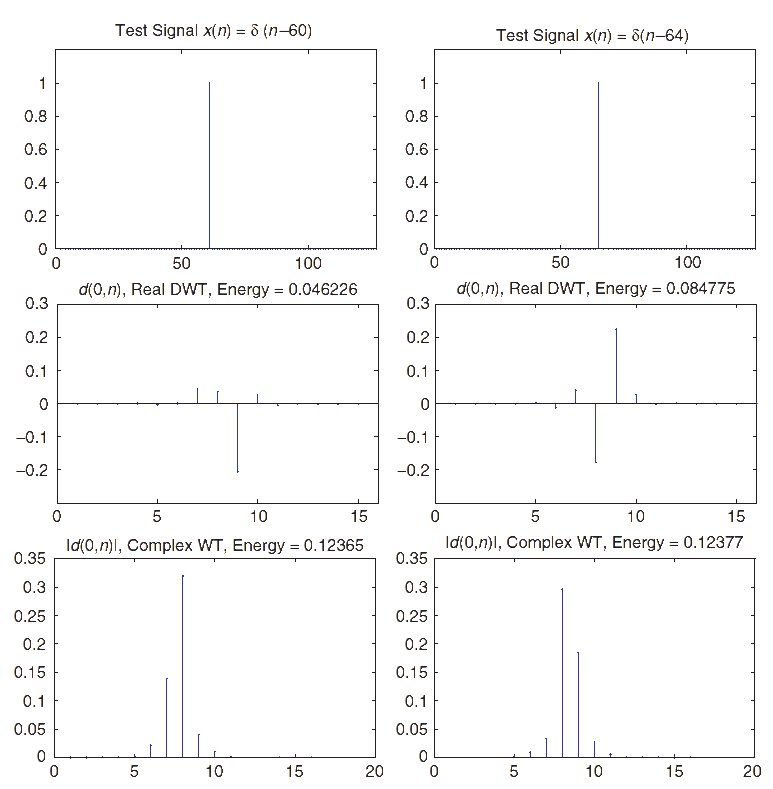
\includegraphics[width=1.1\textwidth]{litreview/images/dwt_zero_crossing.png}
      }
      \mycaption{Sensitivity of DWT coefficients to zero crossings and small
        shifts}{Two impulse signals $\delta(n-60)$ and $\delta(n-64)$ are
        shown (top), as well as the wavelet coefficients for scale $j=1$ for the DWT (middle) and
        for the \DTCWT\ (bottom). In the middle row, not only are the coefficients very different
        from a shifted input, but the energy has almost doubled. As the DWT is an orthonormal
        transform, this means that this extra energy has come from other scales. In comparison, the
      energy of the magnitude of the \DTCWT\ coefficients has remained far more constant, as has the
    shape of the envelope of the output.  Image taken from \citep{selesnick_dual-tree_2005}.}
      \label{fig:dwt_zero_crossing}
  \end{figure}

  \begin{figure}
    \centering
    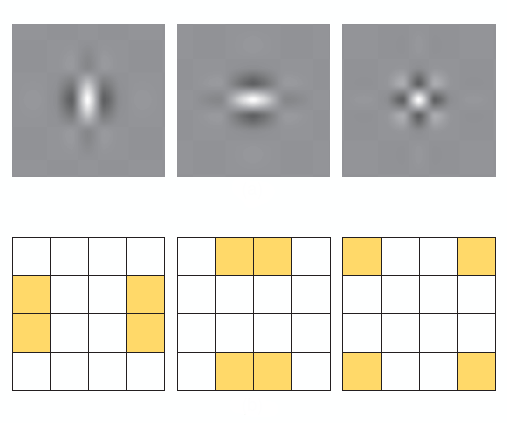
\includegraphics[width=0.7\textwidth]{litreview/images/dwt_wavelets.png}
    \mycaption{Typical wavelets from the 2D separable DWT\@}{Top: Wavelet point
              spread functions for the low-high, high-low, and high-high
              wavelets. High-high wavelets are in a checkerboard pattern, with no
              favoured orientation. Bottom: Idealized support of the spectra of
              each of the wavelets. Image taken from
            \citep{selesnick_dual-tree_2005}.}
      \label{fig:dwt_wavelets}
  \end{figure}

\subsection{Complex Wavelets}\label{sec:complex_wavelets}
  So the DWT has overcome the problem of space-frequency localisation, but it
  has introduced new problems.  Fortunately, we can improve on the DWT with
  complex wavelets, as they can solve these new shortcomings while maintaining
  the desired localization properties. 
  
  The Fourier transform does not suffer from a lack of directional selectivity
  and shift invariance because its basis functions are based on the complex
  sinusoid: 
  \begin{equation} 
    e^{j\omega t} = \cos(\omega t) + j\sin(\omega t)
  \end{equation} 
  whereas the DWT's basis functions are based on only the real
  sinusoid $\cos(\omega t)$\footnote{we have temporarily switched to 1D
  notation here as it is clearer and easier to use, but the results still hold
  for 2D}. As $t$ moves along the real line, the phase of the
  Fourier coefficients change linearly, while their magnitude remains constant. In
  contrast, as $t$ moves along the real line, the sign of the real coefficient
  oscillates between -1 and 1, and its magnitude changes in a non-linear way.

  These nice properties come from the fact that the cosine and sine functions of the
  Fourier transform form a Hilbert Pair, and so together they constitute an 
  analytic signal.

  We can achieve these nice properties if the mother wavelet for our wavelet
  transform is analytic:
  \begin{equation}
    \psi_{c}(t) = \psi_{r}(t) + j\psi_{c}(t) \label{eq:complex_wavelet}
  \end{equation}
  where $\psi_{r}(t)$ and $\psi_{c}(t)$ form a Hilbert Pair (i.e.,\ they are
  $90\degs$ out of phase with each other).

  There are a number of possible ways to do a wavelet transform with complex
  wavelets. We examine two in particular, the Fourier-based method used by
  Mallat et.\ al.\ in their scattering transform
  \citep{bruna_classification_2011, bruna_invariant_2013, bruna_scattering_2013,
  oyallon_generic_2013, oyallon_deep_2015, sifre_rotation_2013,
  sifre_rigid-motion_2014, sifre_rigid-motion_2014-1, sifre_scatnet_2013}, and
  the separable, filter bank based \DTCWT\ developed by Kingsbury
  \citep{kingsbury_wavelet_1997, kingsbury_dual-tree_1998,
  kingsbury_dual-tree_1998-1,  kingsbury_image_1999, kingsbury_shift_1999,
  kingsbury_dual-tree_2000, kingsbury_complex_2001, selesnick_dual-tree_2005}.

\subsection{Fourier Based Wavelet Transform}\label{sec:morlet_fourier}
  The Fourier Based method used by Mallat et.\ al.\ is an efficient
  implementation of the Gabor Transform. Mallat tends to prefer to use a close
  relative of the Gabor wavelet --- the Morlet wavelet --- as the mother wavelet
  for his transform. 
  
  While the Gabor wavelets have the best theoretical trade-off between spatial
  and frequency localization, they have a non-zero mean.  This makes the
  wavelet coefficients non-sparse, as they will all have a DC component to
  them, and makes them inadmissible as wavelets. Instead, the Morlet wavelet
  has the same shape, but with an extra degree of freedom chosen to set $\int
  \psi (\bmu{u}) d\bmu{u} =0$.  This wavelet has equation (in 2D):
  \begin{equation}
    \psi(\bmu{u}) = \frac{1}{2\pi\sigma^2} {(e^{i\bmu{u}\xi} - \beta)}
                     e^{-\frac{|\bmu{u}|^2}{2\sigma^2}} 
    \label{eq:morlet}
  \end{equation}
  where $\beta$ is usually $<<1$ and is this extra degree of freedom, 
  $\sigma$ is the size of the gaussian window, and $\xi$ is the
  location of the peak frequency response --- i.e.,\ for an octave based
  transform, $\xi = 3\pi/4$.

  \Mallat\ add an extra degree of freedom to this by allowing for a non-circular
  gaussian window over the complex sinusoid, which gives control over the angular
  resolution of the final wavelet, so this now becomes:
  \begin{equation}
    \psi(\bmu{u}) = \frac{\gamma}{2\pi\sigma^2}{(e^{i\bmu{u}\xi} - \beta)}
                  e^{-\bmu{u^t}\Sigma^{-1}  \bmu{u}} 
    \label{eq:morlet_slant}
  \end{equation}
  Where
  $$\Sigma^{-1} = \left[ \begin{smallmatrix} 
      \frac{1}{2\sigma^2} & 0 \\ 
      0 & \frac{\gamma^2}{2\sigma^2} 
      \end{smallmatrix} \right] $$
  The effects of modifying the eccentricity parameter $\gamma$ and the window size
  $\sigma$ are shown in \autoref{fig:morlet_filters}. To have a full two
  dimensional wavelet transform, we need to rotate this mother wavelet by angle
  $\theta$ and scale it by $j/Q$, where $Q$ is the number of scales per octave
  (usually 1 in image processing). 
  This can be done by doing the following
  substitutions in \autoref{eq:morlet_slant}:
  \begin{eqnarray*}
    R_{\theta}& = &\left[ \begin{smallmatrix}
                    \cos(\theta) & -\sin(\theta) \\
                    \sin(\theta) & \cos(\theta)
                  \end{smallmatrix} \right] \\
    \bmu{u}_{\theta} & = & R_{-\theta} \bmu{u} \\
    \sigma_j & = & 2^{\frac{j-1}{Q}} \sigma \\
    \xi_j & = & \frac{\xi}{2^{\frac{j-1}{Q}}}
  \end{eqnarray*}
  \Mallat\ combine these two variables into a single coordinate
  \begin{equation}
    \lambda = (\theta, j/Q)
  \end{equation}
  Returning to the higher level notation, we can write
  the Morlet wavelet as the sum of real and imaginary parts: And scaled and
  rotated wavelets as:
  \begin{equation}
    \psi_{\lambda}(\bmu{u}) = 2^{-j/Q}\psi(2^{-j/Q}R_{\theta}^{-1} \bmu{u})
  \end{equation}
  \begin{figure}
    \begin{center}
      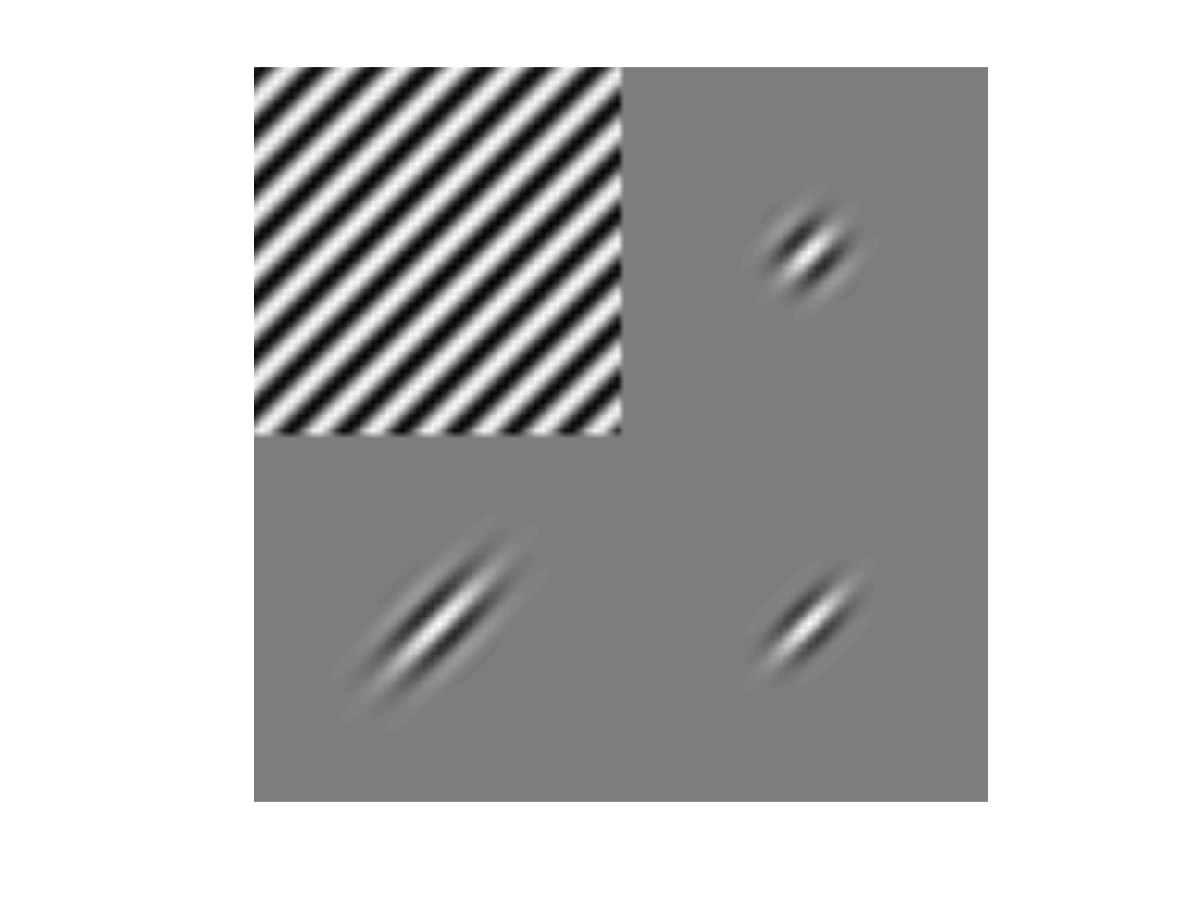
\includegraphics[height=6cm]{litreview/images/morlet_filters.png}
      \mycaption{Single Morlet filter with varying slants and window sizes}
              {Top left --- $45\degs$ plane wave (real part only). Top right --- plane wave with
              $\sigma=3,\gamma=1$. Bottom left --- plane wave with $\sigma=3,\gamma=0.5$. Bottom
            right --- plane wave with $\sigma=2,\gamma=0.5$.}
      \label{fig:morlet_filters}
    \end{center}
  \end{figure}

  \begin{figure}
    \begin{center}
      \makebox[\textwidth][c]{%
        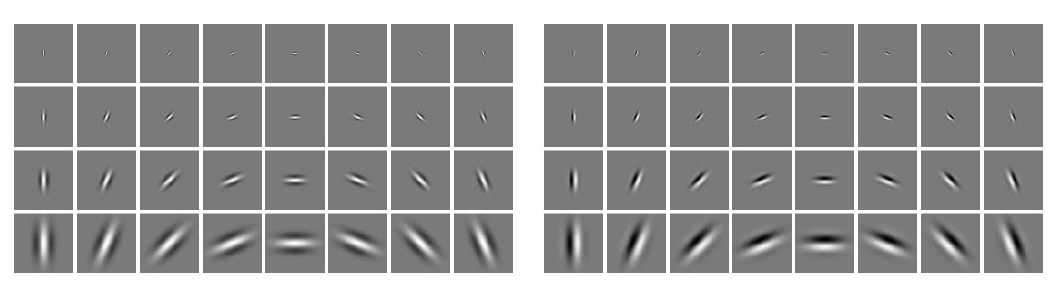
\includegraphics[width=1.1\textwidth]{litreview/images/morlet_wavelets_full.png}
      }
      \mycaption{The full dictionary of Morlet wavelets used by Mallat}
              {The real filters are on the left and the imaginary on the right. The first row
              correspond to scale $j=1$, increasing up to $j=4$. The first column corresponding to
            $\theta = 0$, rotating through $\pi/8$ up to the eighth column of $7\pi/8$,
          $\gamma=1/2$.} 
      \label{fig:morlet_wavelets_full}
    \end{center}
  \end{figure}

\subsubsection{Implementation}\label{sec:morlet_implementation}
  The Fourier Implementation of this Morlet decomposition is shown in
  \autoref{fig:morlet_fourier_process}. It is based on the fact that 
  \begin{equation}
    \mathcal{F}(x \ast \psi)(\omega)
    = \mathcal{F}x(\omega)\mathcal{F}\psi(\omega)
  \end{equation}
  so to compute the family of outputs of $x\ast \psi_{\lambda}$, we can
  precompute the Fourier transform of all of the wavelets, then at run time,
  take the Fourier transform of the image, $x$, multiply with the Fourier
  transform of the wavelets, and then take the inverse Fourier transform of the
  product. The output scale can be chosen by periodizing the product of the
  Fourier transforms, and then compute the inverse Fourier transform at the
  reduced resolution.

  The resulting complexity of the entire operation for an image 
  with $N\x N$ pixels is:
  \begin{itemize}
    \item $O(N^{2} \log N)$ for the forward FFT of $x$.
    \item $O(JLN^{2})$ for the multiplication in the frequency domain. We can see
      this from \autoref{fig:morlet_fourier_process}, there are $J$ scales to
      do multiplication at, and each scale has $L$ orientations, except for the
      low-low.
    \item $O(L \sum_j (2^{-2j}N^{2}) \log {2^{-2j}N^{2}})$ for the inverse FFTs. The
      term inside the sum is just the $O(N^2\log N)$ term of an inverse FFT that
      has been downsampled by $2^j$ in each direction.
  \end{itemize}
  And altogether:
  \begin{equation}
    T(N) = O(N^2 \log N) + O (JLN^{2}) + O(L \sum_{j} N^{2} log 2^{-j} N)
    \label{eq:morlet_efficiency}
  \end{equation}

  \begin{figure}
    \centering
      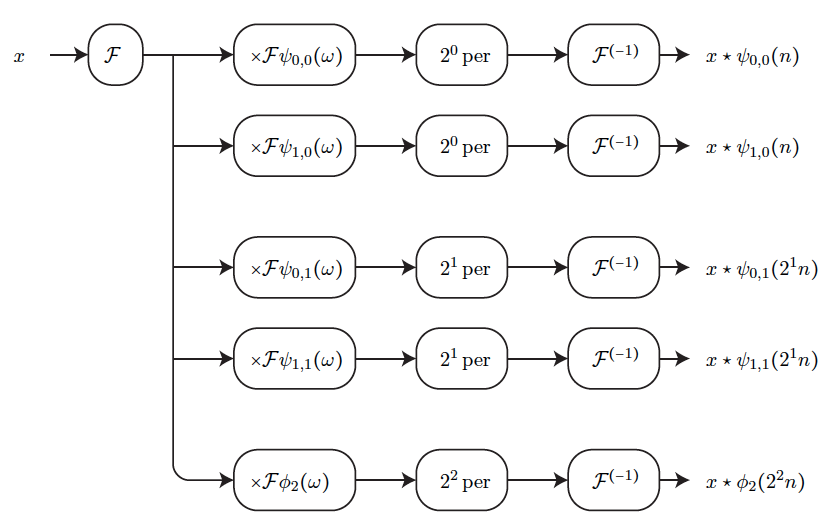
\includegraphics[width=\textwidth]{litreview/images/morlet_fourier_process.png}
      \caption[Fourier Implementation of the Morlet decomposition of an input
              image]
              {Fourier Implementation of the Morlet decomposition of an input
              image, with $J=2$ scales and $L=2$ orientations. The Fourier
              transform of $x$ is calculated and multiplied with the
              (precomputed) Fourier transforms of a bank of Morlet filters. The
              results are periodized according to the target resolution, and
              then the inverse Fourier transform is applied. Image taken from
              \citep{sifre_rigid-motion_2014-1}.}
      \label{fig:morlet_fourier_process}
  \end{figure}

\subsubsection{Invertibility and Energy Conservation}
  We can write the wavelet transform of an input $x$ as 
  \begin{equation}
    \mathcal{W}x = \left\{x \ast \phi_J, x \ast \psi_{\lambda}
    \right\}_{\lambda}
  \end{equation}
  The $\ell^2$ norm of the wavelet transform is then defined by
  \begin{equation}
    \norm{\mathcal{W}x}^2 = \norm{x\ast\phi_J}^2 + \sum_{\lambda}\norm{x \ast
      \psi_\lambda}^2
  \end{equation}
  An energy preserving transform will satisfy Plancherel's equality, so that
  \begin{equation}
    \norm{\mathcal{W}x} = \norm{x}
  \end{equation}
  which is a nice property to have for invertibility, as well as for analysing
  how different signals get transformed (e.g.\ white noise versus standard
  images).
  
  For a transform to be invertible, we examine the measure of how tightly its
  basis functions tile the Fourier plane with its Littlewood-Paley function:  
  \begin{equation}
    A(\omega) = {|\mathcal{F}\phi_J(\omega)|}^2
    + \sum_{\lambda} {|\mathcal{F}\psi_{\lambda}(\omega)|}^2
  \end{equation}
  If the tiliing is $\alpha$-tight, then $\forall \omega \in \mathbb{R}^2$:
  \begin{equation}
    1-\alpha \le A(\omega) \le 1
  \end{equation}
  and the wavelet operator, $\mathcal{W}$ is an $\alpha$ frame. If $A(\omega)$
  is ever close to 0, then there is not a good coverage of the frequency plane
  at that location. If it ever exceeds 1, then there is overlap between bases.
  Both of these conditions make invertibility difficult\footnote{In practise,
  if $A(\omega)$ is only slightly greater 1 for only a few small areas of
  $\omega$, approximate inversion can be achieved}.
  \autoref{fig:morlet_littlewood_paley} show the invertibility of a few
  families of wavelets used by \Mallat. Invertibility is possible, but not
  guaranteed for all configurations. The Fourier transform of the inverse
  filters are defined by:
  \begin{eqnarray}
    \mathcal{F}\phi_J^{-1}(\omega) &=& A(\omega)^{-1} \mathcal{F}\phi_J(\omega) \\
    \mathcal{F}\psi_{\lambda}^{-1}(\omega) &=& A(\omega)^{-1}
      \mathcal{F}\psi_{\lambda}(\omega) 
  \end{eqnarray}

  \begin{figure}
    \centering
      \makebox[\textwidth][c]{%
        % 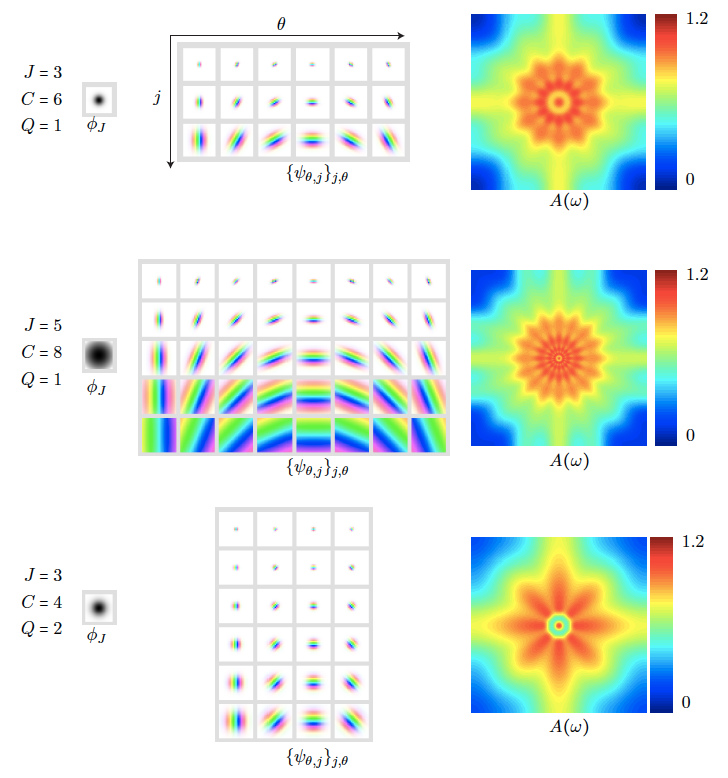
\includegraphics[width=1.1\textwidth]{images/morlet_littlewood_paley.png}
      }
      \caption[Three Morlet Wavelet Families and their tiling of the frequency
              plane]
              {Three Morlet Wavelet Families and their tiling of the frequency
              plane. For each set of parameters, the point spread functions of
              the wavelet bases are shown, next to their Littlewood-Paley sum
              $A(\omega)$. None of the configurations cover the corners of the
              frequency plane, and they often exceed 1. 
              Increasing $J$, $L$ (Sifre uses $C$ in these
              diagrams) or $Q$ gives better frequency localization but at the
              cost of spatial localization and added complexity. Image taken
              from \citep{sifre_rigid-motion_2014-1}.}
      \label{fig:morlet_littlewood_paley}
  \end{figure}


% The discrete wavelet transform (DWT) provides a non-redundant representation
  % of

% signals, hence overcomes the problem of redundancy. The DWT samples the
% timefrequency
% plane and only preserves the least number of the discrete coefficients
% that are required for perfect synthesis. The scale parameter a is sampled first
% on a logarithmic grid, and then the time parameter b is sampled with respect to
% the scale parameter. Though any sampling rate is possible, the DWT is mostly
% computed on the dyadic grid such that the DWT can be efficiently implemented
% by filter bank trees. This is of real value for practical applications.
% Figure 3.1 shows the diagram for a 4-level forward and inverse DWT, which
% explains how the DWT can be efficiently implemented by octave-band,
% discretetime
% filter bank trees. The notations in the diagram have the following meanings:
% 1. x is the original signal
% 2. ˆx is the reconstructed signal
% 3. H0 is the low-pass decomposition filter
% 4. H1 is the high-pass decomposition filter
% 5. °#2 is the operation that downsamples the signal by 2
% 6. G0 is the low-pass reconstruction filter
% 7. G1 is the high-pass reconstruction filter
% 8. °"2 is the operation that upsamples the signal by 2 by inserting zeros
% 9. w(j) are the wavelet coefficients in the j-th subband.
% The decomposition filter (H0, H1) and reconstruction filters (G0, G1) are
% carefully
% chosen in order that the wavelet transform can be inverted, i.e. x = ˆx. The
% above procedure can be represented by matrix-vector notations, which will later
% be introduced in 3.2.3.
% 
\subsection{The \DTCWT}
  The \DTCWT was first proposed by \citeauthor{kingsbury_dual-tree_1998} in
  \cite{kingsbury_dual-tree_1998, kingsbury_dual-tree_1998-1} as a way to combat
  many of the shortcomings of the DWT, in particular, its poor directional
  selectivity, and its poor shift invariance. A thorough analsysis of the
  properties and benefits of the \DTCWT\ is done in
  \cite{kingsbury_image_1999,selesnick_dual-tree_2005}. Building on these
  properties, it been used
  successfully for denoising and inverse problems \cite{rivaz_bayesian_2001,
  zhang_bayesian_2008, zhang_variational_2015, miller_image_2008}, texture
  classification \cite{hatipoglu_texture_1999, rivaz_complex_1999}, image
  registration \cite{loo_motion-estimation-based_2001, chen_efficient_2012}
  and
  SIFT-style keypoint generation matching \cite{fauqueur_multiscale_2006,
  anderson_determining_2005, anderson_rotation-invariant_2006,
  bendale_multiscale_2010, ng_robust_2012} amongst many other applications. 

  Compared to Gabor (or Morlet) image analysis, the authors of
  \cite{selesnick_dual-tree_2005} sum up the dangers as:
  \begin{quote}
    A typical Gabor image analysis is either expensive to compute, is
    noninvertible, or both.
  \end{quote}
  This nicely summarises the difference between this method and the Fourier
  based method outlined in \autoref{sec:morlet_fourier}. The \DTCWT\ is
  a filter bank (FB) based wavelet transform. It is faster
  to implement than the Morlet analysis, as well as being more readily invertible.

\subsubsection{Deisgn Criteria for the \DTCWT}
  It was stated in
  \autoref{sec:complex_wavelets} that if the mother (and daughter) wavelets
  were complex, with their real and imaginary parts forming a Hilbert pair,
  then the wavelet transform of a signal with these $\{\psi_{j,n}\}_{j,n}$
  would give a representation that had nice shift properties\footnote{in
  particular, that a shift in input gives the same shift in magnitude of the
  wavelet coefficients, and a linear phase shift}, was insensitive to zero crossings of the
  wavelet, and had good directional selectivity. 
  
  As in \autoref{sec:complex_wavelets}, we want to have a complex mother
  wavelet $\psi_c$ that satisfies \autoref{eq:complex_wavelet}, but now
  achieved with filter banks. A slight deviation from standard filter bank
  notation, where $h_0, h_1$ are the analysis and $g_0,g_1$ are the synthesis
  filters. We define:
  \begin{itemize}
    \item $h_0, h_1$ the low and high-pass analysis filters for $\psi_r$ (henceforth called
      $\psi_h$)
    \item $g_0, g_1$ the low and high-pass analysis fitlers for $\psi_i$
      (henceforth called $\psi_g$)
    \item $\tilde{h}_0, \tilde{h}_1$ the low and high-pass synthesis filters
      for $\tilde{\psi}_h$.
    \item $\tilde{g}_0, \tilde{g}_1$ the low and hig pass synthesis filters for
      $\tilde{\psi}_g$.
  \end{itemize}

  The dilation and wavelet equations for a 1D filter bank implementation are:
  \begin{eqnarray}
    \phi_h(t) & = & \sqrt{2} \sum_n h_0(n) \phi_h(2t-n) \\
    \psi_h(t) & = & \sqrt{2} \sum_n h_1(n) \phi_h(2t-n) \\
    \phi_g(t) & = & \sqrt{2} \sum_n g_0(n) \phi_g(2t-n) \\
    \psi_g(t) & = & \sqrt{2} \sum_n g_1(n) \phi_g(2t-n) 
  \end{eqnarray}
  This implementation is shown in \autoref{fig:dtcwt_1d_fb}.

  \begin{figure}
    \centering
      % 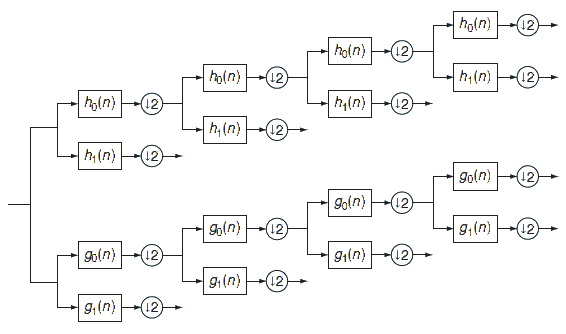
\includegraphics[width=\textwidth]{images/dtcwt_1d_fb.png}
      \caption[Analysis FB for the \DTCWT]
              {Analysis FB for the \DTCWT\@. Top `tree' forms the real
              component of the complex wavelet $\psi_r$, and the bottom tree forms the
              imaginary (Hilbert pair) component $\psi_i$. Image taken from
              \citep{selesnick_dual-tree_2005}.}
      \label{fig:dtcwt_1d_fb}
  \end{figure}

  Designing a filter bank implementation that results in Hilbert symmetric
  wavelets does not appear to be an easy task. However, it was shown
  by \citet{kingsbury_image_1999} (and later proved by
  \citet{selesnick_hilbert_2001}) that the necessary conditions are
  conceptually very simple. One low-pass filter must be a \emph{half-sample shift} of
  the other. I.e.,\ 
  \begin{equation}
    g_0(n) \approx h_0(n-0.5) \rightarrow \psi_g(t) \approx
    \mathcal{H}\{\psi_h(t)\}
  \end{equation}
  As the \DTCWT\ is designed as an invertible filter bank implementation, this
  is only one of the constraints. Naturally, there are also:
  \begin{itemize}
    \item Perfect reconstruction
    \item Finite support
    \item Linear phase
    \item Many vanishing moments at $z=-1$ for good stopband properties
  \end{itemize}
  to consider when building the $h$'s and $g$'s.
  The derivation of the filters that meet these conditions is covered in
  detail in \citep{kingsbury_complex_2001, kingsbury_design_2003}, and in
  general in \citep{selesnick_dual-tree_2005}. The result is the
  option of three families of filters:  biorthogonal filters ($h_0[n] =
  h_0[N-1-n]$ and $g_0[n] = g_0[N-n]$), q-shift filters ($g_0[n]
  = h_0[N-1-n]$), and common-factor filters.

\subsubsection{The Resulting Wavelets and their Properties}
  While analytic wavelets in 1D are useful for their shift invariance, the real
  beauty of the \DTCWT\ is in its ability to make a separable 2D wavelet
  transform with oriented wavelets. 
  
  \autoref{fig:dwt_hh} shows the spectrum of
  the wavelet when the separable product uses purely real wavelets, as is the
  case with the DWT\@. \autoref{fig:dtcwt_hh} however, shows the separable
  product of two complex, analytic wavelets resulting in a localized and
  oriented 2D wavelet.  
  
  I.e.,\ for the $+45\degs$ wavelet\footnote{note that \autoref{fig:dtcwt_hh}
  shows the $135\degs$ wavelet} (which is high
  in both $\omega_1$ and $\omega_2$), the separable product is:
  \begin{eqnarray}
    \psi(\omega_1,\omega_2) & = & \psi_c (\omega_1) \overline{\psi_c
      (\omega_2) } \label{eq:wavelet_separable_product}\\
    & = & (\psi_h(\omega_1) + j \psi_g(\omega_1) \overline{\left(\psi_h(\omega_2)
      + \psi_g(\omega_2) \right)} \nonumber\\
    & = & \psi_h(\omega_1) \psi_h(\omega_2) + \psi_g(\omega_1)
      \psi_g(\omega_2)\nonumber\\
    &&  + j\left( \psi_g(\omega_1) \psi_h(\omega_2) - \psi_h(\omega_1)
        \psi_g(\omega_2) \right)  \label{eq:dtcwt_2d_product}
  \end{eqnarray}
  Similar equations can be obtained for the other five wavelets and the scaling
  function, by replacing
  $\psi$ with $\phi$ for both directions, and not taking the complex conjugate
  in \autoref{eq:wavelet_separable_product} to get the right hand side of the
  frequency plane. 
  
  \autoref{fig:dtcwt_wavelets} shows the resulting wavelets both in the spatial
  domain and their idealized support in the frequency domain.

  \autoref{fig:dtcwt_shift_invariance} shows how the \DTCWT\ compares with the
  DWT with a shifting input.

  \begin{figure}
%      \centering
      \subfloat[]{\makebox[\textwidth][c]{%
        % 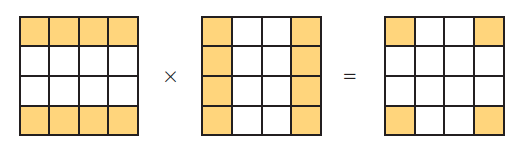
\includegraphics[width=0.8\textwidth]{images/dwt_hh.png}
        \label{fig:dwt_hh}}}
      \newline
      \subfloat[]{\makebox[\textwidth][c]{%
        % 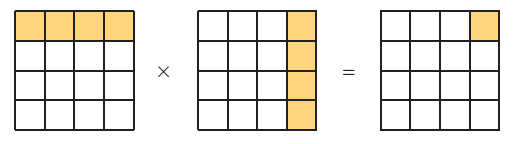
\includegraphics[width=0.8\textwidth]{images/dtcwt_hh.png}
        \label{fig:dtcwt_hh}}}
      \caption[The DWT high-high vs the \DTCWT\ high-high frequency support]
              {\subref{fig:dwt_hh} The high-high DWT wavelet having a passband in
              all 4 corners of the frequency plane vs \subref{fig:dtcwt_hh} the
              high-high \DTCWT\ wavelet frequency support only existing in one
              quadrant. Taken from \citep{selesnick_dual-tree_2005}}
      \label{fig:dwt_dtcwt_hh}
  \end{figure}

  \begin{figure}
    \centering
      % 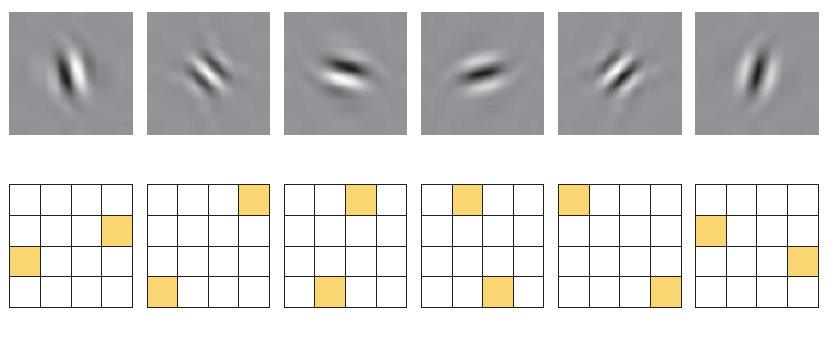
\includegraphics[width=\textwidth]{images/dtcwt_wavelets.png}
      \caption[Wavelets from the 2D \DTCWT]
              {Wavelets from the 2d \DTCWT\@. \textbf{Top:} The six  oriented filters
      in the space domain (only the real wavelets are shown). \textbf{Bottom:}
      Idealized support of the Fourier spectrum of each wavelet in the 2D
      frequency plane. Spectra of the the real wavelets are shown --- the
      spectra of the complex wavelets ($\psi_h + j\psi_g$) only has support in the top
      half of the plane. Image taken from \citep{selesnick_dual-tree_2005}.}
      \label{fig:dtcwt_wavelets}
  \end{figure}
  \begin{figure}
    \centering
      \makebox[\textwidth][c]{%
        % 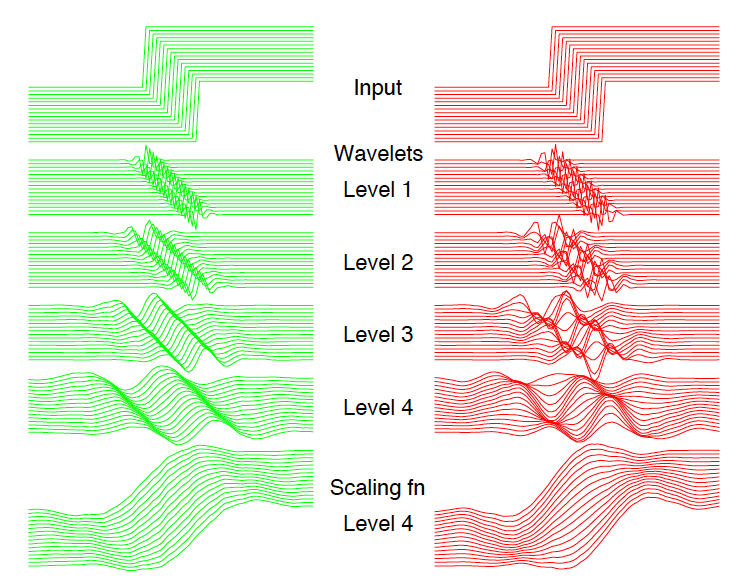
\includegraphics[width=1.1\textwidth]{images/dtcwt_shift_invariance.png}
      }
      \caption[The shift invariance ofthe \DTCWT\ vs.\ the real DWT]
              {The shift invariance of the \DTCWT\ (left) vs.\ the real DWT
              (right). The \DTCWT\ linearizes shifts in the phase change of the complex
              wavelet. Image taken from \citep{kingsbury_dual-tree_1998}.}
      \label{fig:dtcwt_shift_invariance}
  \end{figure}

\subsubsection{Implementation and Efficiency}\label{sec:dtcwt_efficiency}
  \autoref{fig:dtcwt_1d_fb} showed the layout for the \DTCWT\ for 1D signals. We
  saw from \autoref{eq:dtcwt_2d_product} that the 2D separable product of wavelets
  involved the product of $\psi_g$, $\psi_h$, $\phi_g$, and $\phi_h$ terms, with
  some summing and differencing operations. \autoref{fig:dtcwt_fb} shows how to
  efficiently implement this with FBs.
  
  \begin{figure}
    \centering
    \makebox[\textwidth][c]{%
      % 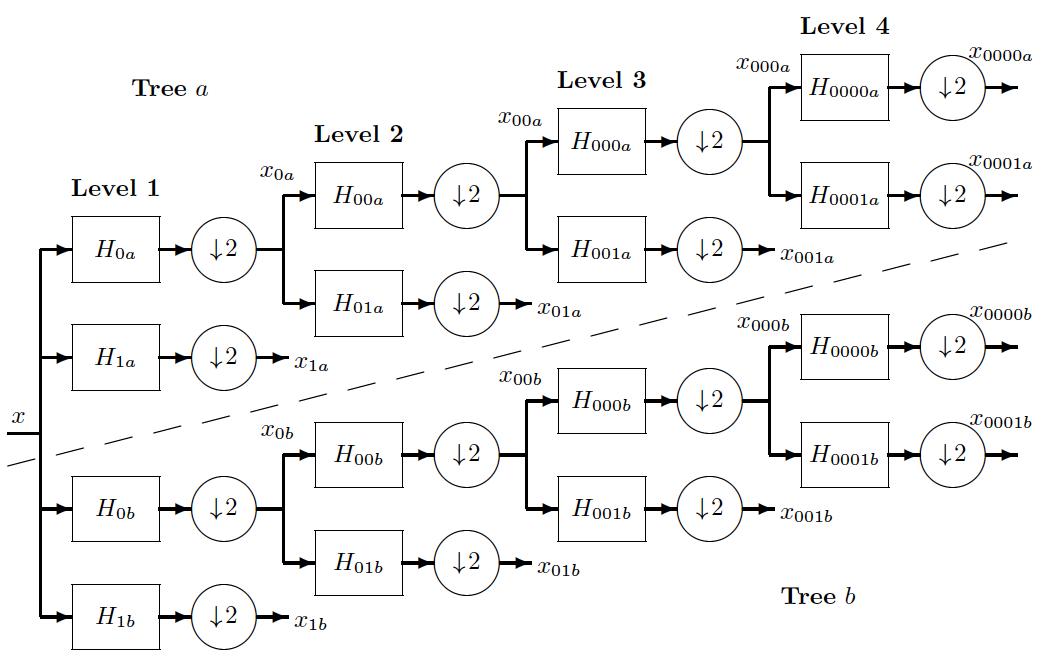
\includegraphics[width=1.1\textwidth]{images/dtcwt_fb.png}
    }
      \caption[The filter bank implementation of the \DTCWT]
              {The filter bank implementation of the \DTCWT\@. Image taken from 
              \citep{kingsbury_image_1999}}
      \label{fig:dtcwt_fb}
  \end{figure}

  As we did for \autoref{sec:morlet_implementation}, we calculate and compare
  the complexity of the \DTCWT\@. To do this, we must know the length of our
  $h$ and $g$ filters. It is also important to know that we must use different
  filters for the first scale to the deeper scales, as this achieves better
  analyticity. A typical configuration will use biorthogonal filters for the
  first scale, then qshift for subsequent scales.
  % The \emph{nearly symmetric type a} biorthogonal filters for the first level, and then the \emph{qshift type b}
  % filters for the deeper levels of the transform. 
  These filters have the following number of taps\footnote{This implementation
  uses the shorter near\_sym\_a biorthogonal filters and qshift\_a filters.
  Smoother wavelets can have slightly more taps}:
  % \begin{table}
    \begin{center}
    \begin{tabular}{ccccc} \hline
                   & $h_0$ & $h_1$ & $g_0$ & $g_1$ \\\hline
      biorthogonal & 5     & 7     & 7     & 5     \\
      qshift       & 10    & 10    & 10    & 10      
    \end{tabular}
    \end{center}
  % \end{table}
  The resulting complexity of the entire forward wavelet transform for an image
  with $N\x N$ pixels is:
  \begin{itemize}
    \item First layer (Image size $=N\x N$):
      \begin{itemize}
        \item Column filtering requires $5N^2+7N^2$ multiply-adds
        \item Row filtering to make the LoLo term requires $5N^2$ more
          multiply-adds
        \item Row filtering to make $15\degs$ and $165\degs$ requires
          $5N^2+4N^2$
          multiply-adds (the 4 here comes from the $\Sigma/\Delta$ function
          block in \autoref{fig:dtcwt_fb}).
        \item Row filtering to make the $45\degs$ and $135\degs$ requires $7N^2
          +4N^2$ multiply-adds
        \item Row filtering to make the $75\degs and 105\degs$ requires
          $7N^2+4N^2$
          multiply-adds
      \end{itemize}
      The total being 
      $$T(N) = (5+7+5+5+4+7+4+7+4)N^2 = 48N^2$$
    \item Second and deeper layers (Image size $=2^{-j}N\x 2^{-j}N=M\x M$):
      \begin{itemize}
        \item Column filtering requires $10M^2+10M^2$ multiply-adds
        \item Row filtering to make the LoLo term requires $10M^2$ more
          multiply-adds
        \item Row filtering to make $15\degs$ and $165\degs$ requires
          $10M^2+4M^2$
          multiply-adds (the 4 here comes from the $\Sigma/\Delta$ function
          block in \autoref{fig:dtcwt_fb}).
        \item Row filtering to make the $45\degs$ and $135\degs$ requires
          $10M^2 +4M^2$ multiply-adds
        \item Row filtering to make the $75\degs$ and $105\degs$ requires
          $10M^2+4M^2$
          multiply-adds
      \end{itemize}
      The total being: 
      $$T(M) = (10+10+10+10+4+10+4+10+4)M^2 = 68M = 68\x 2^{-2j}N^2$$
  \end{itemize}
  \begin{equation}
    T(N) = 48N^2 + \sum_{j=1}^{J} 68 \x 2^{-2j}N^2 \approx 100N^2
  \end{equation}
  As the term $\sum_{j=1}^{J} 68 \x 2^{-j}$ is a geometric series that sums to
  $1/3$ as $j \rightarrow \infty$. We have also rounded up the sum to be conservative.

  It is difficult to compare this with the complexity of the Fourier-based
  implementation of the Morlet wavelet transform we have derived in
  \autoref{sec:morlet_implementation}, as we cannot readily estimate the big-O
  order constants for the 2D FFT method. However, the central term, $JLN^2$,
  would cost $24N^2$ multiplies for four scales and six orientations. These are
  complex multiplies, as they are in the Fourier domain, which requires
  four real multiplies. On top of this, to account for the periodic repetition 
  of the inverse FFT implementation, Mallat et.\ al.\ symmetrically extend the image by
  $N/2$ in each direction. This means that the central term is already on the
  order of $\sim 200N^2$ multiplies, without even considering the more
  expensive forward and inverse FFTs. 

  For a simple comparison experiment, we performed the two transforms on a four
  core Intel i7 processor (a moderately high-end personal computer). The
  \DTCWT\ transform took roughly 0.15s on a black and
  white $32\x 32$ image, vs. 0.5s for the Fourier-based method. For a larger,
  $512\x 512$ image, the \DTCWT\ implementation took 0.35s vs. 3.5s
  (times were averaged over several runs).
  
\subsubsection{Invertibility and Energy Conservation}
  We analysed the Littlewood-Paley function for the Morlet-Fourier
  implementation, and saw what areas of the spectrum were better covered than
  others. How about for the \DTCWT\@?

  It is important to note that in the case of the \DTCWT\, the wavelet
  transform is also approximately unitary, i.e.,\
  \begin{equation}
    \norm{x}^2 \approx \norm{\mathcal{W}x}^2
  \end{equation}
  and the implementation is perfectly invertible as the Littlewood-Paley
  function is unity (or very near unity) $\forall \omega$. See
  \autoref{fig:dtcwt_lwoodpaley}. This is not a surprise, as it is a design
  constraint in choosing the filters, but nonetheless is important to note. 

  A beneficial property of energy conservation is that the noise in the input
  will equal the noise in the wavelet coefficients. When we introduce
  Scatternets, we can show that we can keep the unitary property in the
  scattering coefficients. This is an important property, particularly in light
  of the recent investigations in \citep{szegedy_intriguing_2013}. This paper
  saw that it is easy to find cases in CNNs where a small amount of input
  perturbation results in a completely different class label (see
  \autoref{fig:difference}). Having a unitary transform limits the
  amount the features can change, which will make the entire network more
  stable to distortion and noise.

  \begin{figure}
    \subfloat{\makebox[0.6\textwidth][c]{%
      % 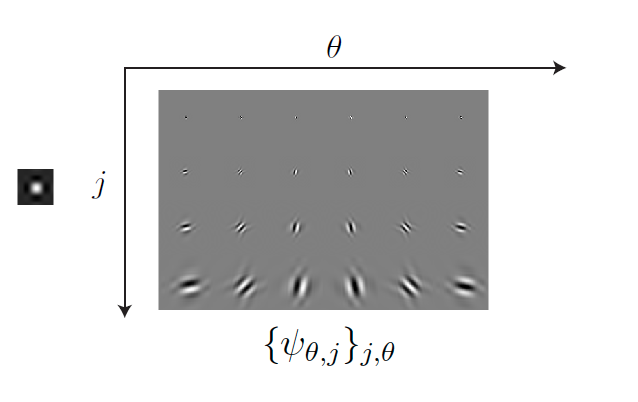
\includegraphics[width=0.7\textwidth,valign=c]{images/dtcwt_real_4scales.png}
    }}
    \subfloat{\makebox[0.4\textwidth][c]{%
      % 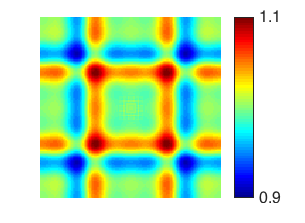
\includegraphics[width=0.5\textwidth,valign=c]{scripts/dtcwt_lwoodpaley_2.png}
    }}
    \caption[\DTCWT\ basis functions and their frequency coverage]
    {Four scales of the \DTCWT\ (left) and its associated frequency
    coverage, or $A(\omega)$ (right). Note the reduced scale compared to \autoref{fig:morlet_littlewood_paley}.}
    \label{fig:dtcwt_lwoodpaley}
  \end{figure}

  \begin{figure}
    \centering
    % 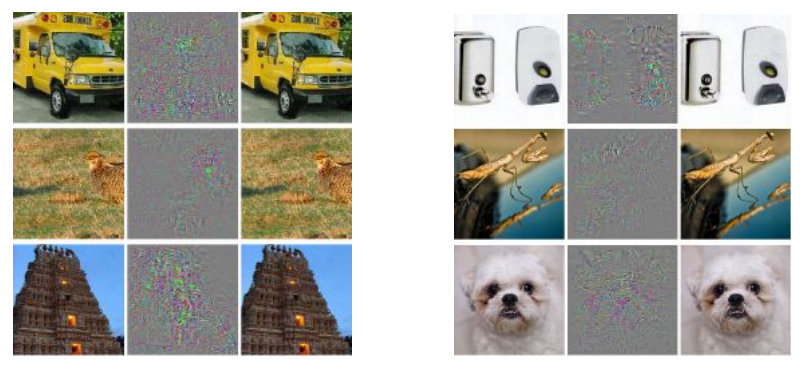
\includegraphics[width=0.9\textwidth]{images/adversarial_nets.png}
    \caption[Two adversarial examples generated for AlexNet]
    {Two adversarial examples generated for AlexNet. The left column
    shows a correctly predicted sample, the right column an incorrectly
    predicted example, and the centre column the difference between the two
    images, magnified 10 times. Image taken from
    \citep{szegedy_intriguing_2013}.}
    \label{fig:difference}
  \end{figure}
\subsection{Summary of Methods}
  One final comparison to make between the \DTCWT\ and the Morlet wavelets is
  their frequency coverage. The Morlet wavelets can be made to be tighter than
  the \DTCWT, which gives better angular resolution --- see
  \autoref{fig:wavelet_freq_resp}. However it is not always
  better to keep getting finer and finer resolutions, indeed the Fourier
  transform gives the ultimate in angular resolution, but as mentioned, this
  makes it less stable to shifts and deformations. 

  \autoref{tab:dtcwt_vs_dwt_vs_mallat} compares the advantages and
  disadvantages of the wavelet methods discussed in this chapter.

  \begin{figure}
    \subfloat[\DTCWT\ wavelets (left to right) --- $15\degs$, $45\degs$ and $75\degs$]{%
      \makebox[\textwidth][c]{%
      % 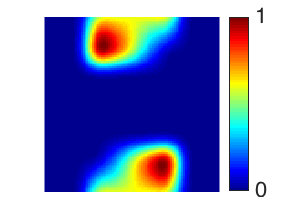
\includegraphics[width=0.4\textwidth]{scripts/dtcwt_15deg_energy.png}
      % 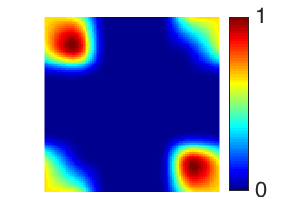
\includegraphics[width=0.4\textwidth]{scripts/dtcwt_45deg_energy.png}
      % 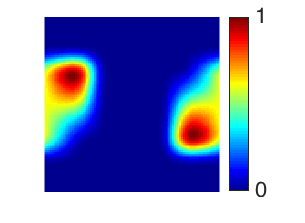
\includegraphics[width=0.4\textwidth]{scripts/dtcwt_75deg_energy.png}
    }}
    \newline
    \subfloat{%
      \makebox[\textwidth][c]{%
      % 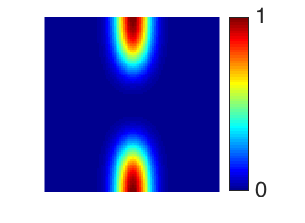
\includegraphics[width=0.4\textwidth]{scripts/mallat_0deg_energy.png}
      % 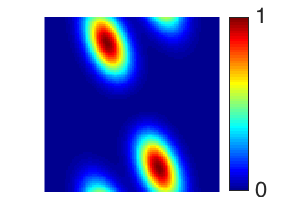
\includegraphics[width=0.4\textwidth]{scripts/mallat_225deg_energy.png}
      % 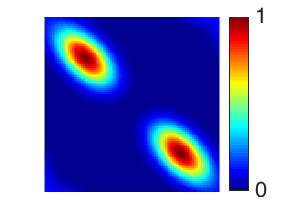
\includegraphics[width=0.4\textwidth]{scripts/mallat_45deg_energy.png}
    }}
    \newline
    \subfloat[Morlet wavelets (left to right) --- $0\degs$, $22.5\degs$, $45\degs$, 
              $67.5\degs$,  and $90\degs$]{%
      % Use two makebox commands to center the images
      \makebox[0.5\textwidth][c]{%
        \hspace{1cm}
        % 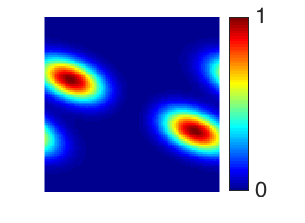
\includegraphics[width=0.4\textwidth,center]{scripts/mallat_675deg_energy.png}
      }
      \makebox[0.5\textwidth][c]{%
        \hspace{-1cm}
        % 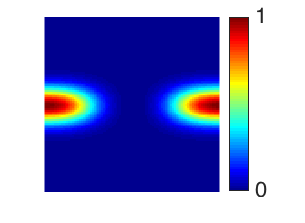
\includegraphics[width=0.4\textwidth,center]{scripts/mallat_90deg_energy.png}
      }
    }
    \caption[Comparison of the energy spectra for \DTCWT\ wavelets to Morlet
    wavelets]
    {Normalized Energy spectra of the \DTCWT\ wavelets versus the preferred
            8 orientation Morlet wavelets by Mallat for the second quadrant.
            Orientations listed refer to the edge orientation in the spatial
            domain that gives the highest response. All wavelets have been
            normalized to be between zero and one.
            The Morlet wavelets have finer angular
            resolution, which can give better discrimination, at the cost of
            decreasing stability to deformations, and requiring larger spatial
            support.}
    \label{fig:wavelet_freq_resp}
  \end{figure}
\begin{table}[h]
  \caption{A comparison of wavelet transform methods}
  \label{tab:dtcwt_vs_dwt_vs_mallat}
  \begin{center}

  \begin{tabularx}{\textwidth}[t]{X|X|X} \toprule
      DWT & \DTCWT\ & FFT-based\\ \hline
      
      \cellcolor{green!25} Efficient filter bank implementation & 
        \cellcolor{green!25 }Efficient filter bank implementation &
        \cellcolor{red!25} Convolutions done in the frequency domain \\ \hline
      \cellcolor{green!25}$O(N)$ & 
        \cellcolor{green!25}$O(N)$ & 
        \cellcolor{red!25}$O(N\log N)$ \\ \hline
      \cellcolor{green!25}Perfect reconstruction inherent to the design & 
        \cellcolor{green!25}Perfect reconstruction inherent to the design & 
        \cellcolor{red!25}Perfect reconstruction possible, but not inherent \\ \hline
      \cellcolor{green!25}Energy preserving & 
        \cellcolor{green!25}Energy preserving & 
        \cellcolor{green!25}Energy preserving \\ \hline
      \cellcolor{green!25}Critically sampled & 
        \cellcolor{red!25}Tight frame, with $4:1$ redundancy & 
        \cellcolor{red!25}Tight frame, with variable redundancy (often around
        $4:1$ in implenetations by \Mallat) \\ \hline
      \cellcolor{red!25}Purely real wavelets & 
        \cellcolor{green!25}Complex, analytic wavelets & 
        \cellcolor{green!25}Complex, analytic wavelets \\ \hline
      \cellcolor{red!25}Poorly Oriented & 
        \cellcolor{green!25}Well oriented & 
        \cellcolor{green!25}Well oriented \\ \hline
      \cellcolor{red!25}Fixed number of bandpass wavelets & 
        \cellcolor{red!25}Fixed number of bandpass wavelets & 
        \cellcolor{green!25}Flexible number of bandpass wavelets \\ \hline
      \cellcolor{red!25}Oversampling costly (at odds with the algorithm) & 
        \cellcolor{red!25}Oversampling costly (at odds with the design) & 
        \cellcolor{green!25}Oversampling only linearly more expensive \\
      \cellcolor{green!25}Can use symmetric extension for the edges of images &
        \cellcolor{green!25}Can use symmetric extension for the edges of images &
        \cellcolor{red!25}Assumes periodic extension of signals \\
      \bottomrule
  \end{tabularx}
  \end{center}
\end{table}
